\documentclass[10pt]{scrreprt}
\usepackage[a4paper, top=30mm, left=25mm, right=25mm, bottom=30mm]{geometry}
\usepackage[utf8]{inputenc}

\usepackage[Bjornstrup]{fncychap}
\usepackage{ngerman}
\usepackage{graphicx}
\usepackage{epstopdf}
\usepackage{etoolbox}
\usepackage{enumitem}
\usepackage{url}
\usepackage{numprint}
\usepackage{longtable}
\usepackage{tabu}
\usepackage{multirow}
\usepackage{caption}
\usepackage{array}
\usepackage{listings}
\usepackage{amssymb}


\makeatletter
\patchcmd{\@makechapterhead}{\vspace*{50\p@}}{\vspace*{-20\p@}}{}{}
\patchcmd{\@makeschapterhead}{\vspace*{50\p@}}{\vspace*{7\p@}}{}{}
\patchcmd{\DOTIS}{\vskip 40\p@}{\vskip -12\p@} 
\makeatother
  
\captionsetup[figure]{labelfont={sf,bf},textfont={sf}}
\deffootnotemark{[\thefootnotemark]}
\deffootnote{1.5em}{1em}{[\thefootnotemark] }
\setlength{\parindent}{0pt}
\renewcommand{\labelitemi}{ \raisebox{0.3ex}{\small$\blacktriangleright$} }
\lstset{language=Java}

\newcommand{\sfbf}[1]{\textbf{\sffamily #1}}
\newcommand{\sfit}[1]{\textit{\sffamily #1}}
\newcommand{\W}{\sfbf{W}}
\newcommand{\ziel}[1]{{\fontsize{9.5}{11}\textsf{/#1/}}}
\newcommand{\ziellabel}{Z}
\newcommand{\muss}{\renewcommand{\labelenumi}{\textbf{\ziel{\ziellabel\numprint{\theenumi}0}}}}
\newcommand{\wunsch}{\renewcommand{\labelenumi}{\textbf{\ziel{\ziellabel\numprint{\theenumi}0W}}}}
\newcommand{\JoglEarth}{\raisebox{-1.2mm}{
\includegraphics[scale=0.33]{Logo-Text.eps}} }
\newcommand{\textref}[1]{\mbox{\raisebox{0.1ex}{\small$\rightarrow$ }\textit{#1}}}

\newenvironment{details}[1][6pt]{%
  \parskip#1 \parindent6mm \raggedright%
  \def\item{\par\ignorespaces\hangindent=5mm \hangafter1}}{%
  \par\ignorespaces} 
  

\begin{document}

\thispagestyle{empty}
\sffamily
 
\title{Entwurf}

\begin{figure}
\begin{flushright}
	
\includegraphics[scale=0.4]{uniLogo.eps}
\vspace{2.0 cm}
\end{flushright}
\end{figure}

\begin{center}
\vspace{2.0 cm}
{\LARGE SEP – Wintersemester 2013/14}

\vspace{1.0 cm}
\textbf{{\Huge Entwurf}}

\vspace{0.8 cm}
\begin{figure}[!htb]
\begin{center}
	%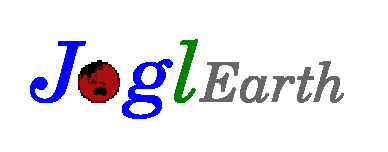
\includegraphics[scale=1.0]{projektLogo.eps}
	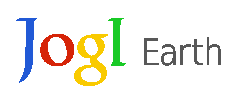
\includegraphics[scale=1.5]{Logo-Print.eps}
\end{center}
\end{figure}

\vspace{0.2 cm}
\textbf{{\huge OpenStreetMap: Die Welt in 3D}}

\vspace{1.5 cm}
08.11.2013

\vspace{0.5 cm}
Version: 1.0

\vspace{1.5 cm}
{\Large Projektbetreuer: Peter Barth}

\vspace{1.5 cm}
\begin{tabular}{|c|c|c|}
\hline 
\rule[-1ex]{0pt}{4ex} \textbf{Phase} & \textbf{Verantwortlicher} & \textbf{E-Mail Adresse} \\ 
\hline  \hline
\rule[-1ex]{0pt}{4ex} Pflichtenheft & Gabriele Haas & haasgab@fim.uni-passau.de \\ 
\hline  \hline
\rule[-1ex]{0pt}{4ex} Entwurf & Thomas Eder & ederthom@fim.uni-passau.de \\ 
\hline  \hline
\rule[-1ex]{0pt}{4ex} Spezifikation & Christof Blauberger & blauberg@fim.uni-passau.de \\ 
\hline  \hline
\rule[-1ex]{0pt}{4ex} Implementierung & Fabian Knorr & knorrfab@fim.uni-passau.de \\ 
\hline \hline 
\rule[-1ex]{0pt}{4ex} Testing & Constantin Wenger & wengerco@fim.uni-passau.de \\ 
\hline  \hline
\rule[-1ex]{0pt}{4ex} Präsentation & Sebastian Reichl & reichlse@fim.uni-passau.de \\ 
\hline 
\end{tabular}

\end{center}


\pagebreak
\rmfamily
\tableofcontents

\chapter{Einleitung}

Dieses Dokument stellt den Entwurf von \JoglEarth und der einzelnen Klassen mit deren Interaktion vor.
Die geforderten Funktionalitäten aus dem Pflichtenheft sind abgebildet.
\textbf{Abweichungen zum Pflichtenheft hier begründen}
\\

Im Zuge der Erstellung dieses Dokuments erfolgte die Planung aller Komponenten mit deren zugehörigen Funktionen. Um das Programm im ganzen zu erfassen finden verschiedene Darstellungsarten Anwendung. \\

Als Überblick wird das Konzept des Programms zu Beginn mithilfe eines Architekturdiagramms erklärt. \\

Der \textit{Rational Software Architect} visualisiert die Interaktionen unter den Komponenten in Form von Diagrammen. Aus den Grafiken gehen einerseits die Vererbungshierachien, andererseits die angewendeten Design Patterns hervor. \\

Der innere Aufbau der Klassen, wie z.B. deren Methoden, wird anhand eines Klassendiagramms verdeutlicht. Wichtige Komponenten sind zusätzlich gesondert herausgearbeitet. \\ 

Um komplexere Zusammenhänge zu veranschaulichen werden detaillierte Auszüge aus der Klassenstruktur entnommen und in einzelne Sequenzdiagramme umgesetzt. Diese erläutern die interne Kommunikation und geben einen Überblick, zu welchem Zeitpunkt im Programmablauf eine oder mehrere Instanzen einer Komponente existiert. \\

Die Priorisierung der im Pflichtenheft angeführten Qualitätsbestimmungen besagt, dass Stabilität, Fehlertoleranz und effizientes Speichermanagement die Hauptmerkmale von \JoglEarth darstellen. Das Code Design wird den Anforderungen der Qualitätskriterien gerecht.\\  

Um dem heutigen Standard hoher Softwarequalität sicherzustellen, fließen im gesamten Entwurfsprozess die gesetzten Gütekriterien und Qualitätsmerkmale ein. 

\chapter{UML-Klassendiragramme}

\section{Package Model}
\begin{figure}[!htb]
	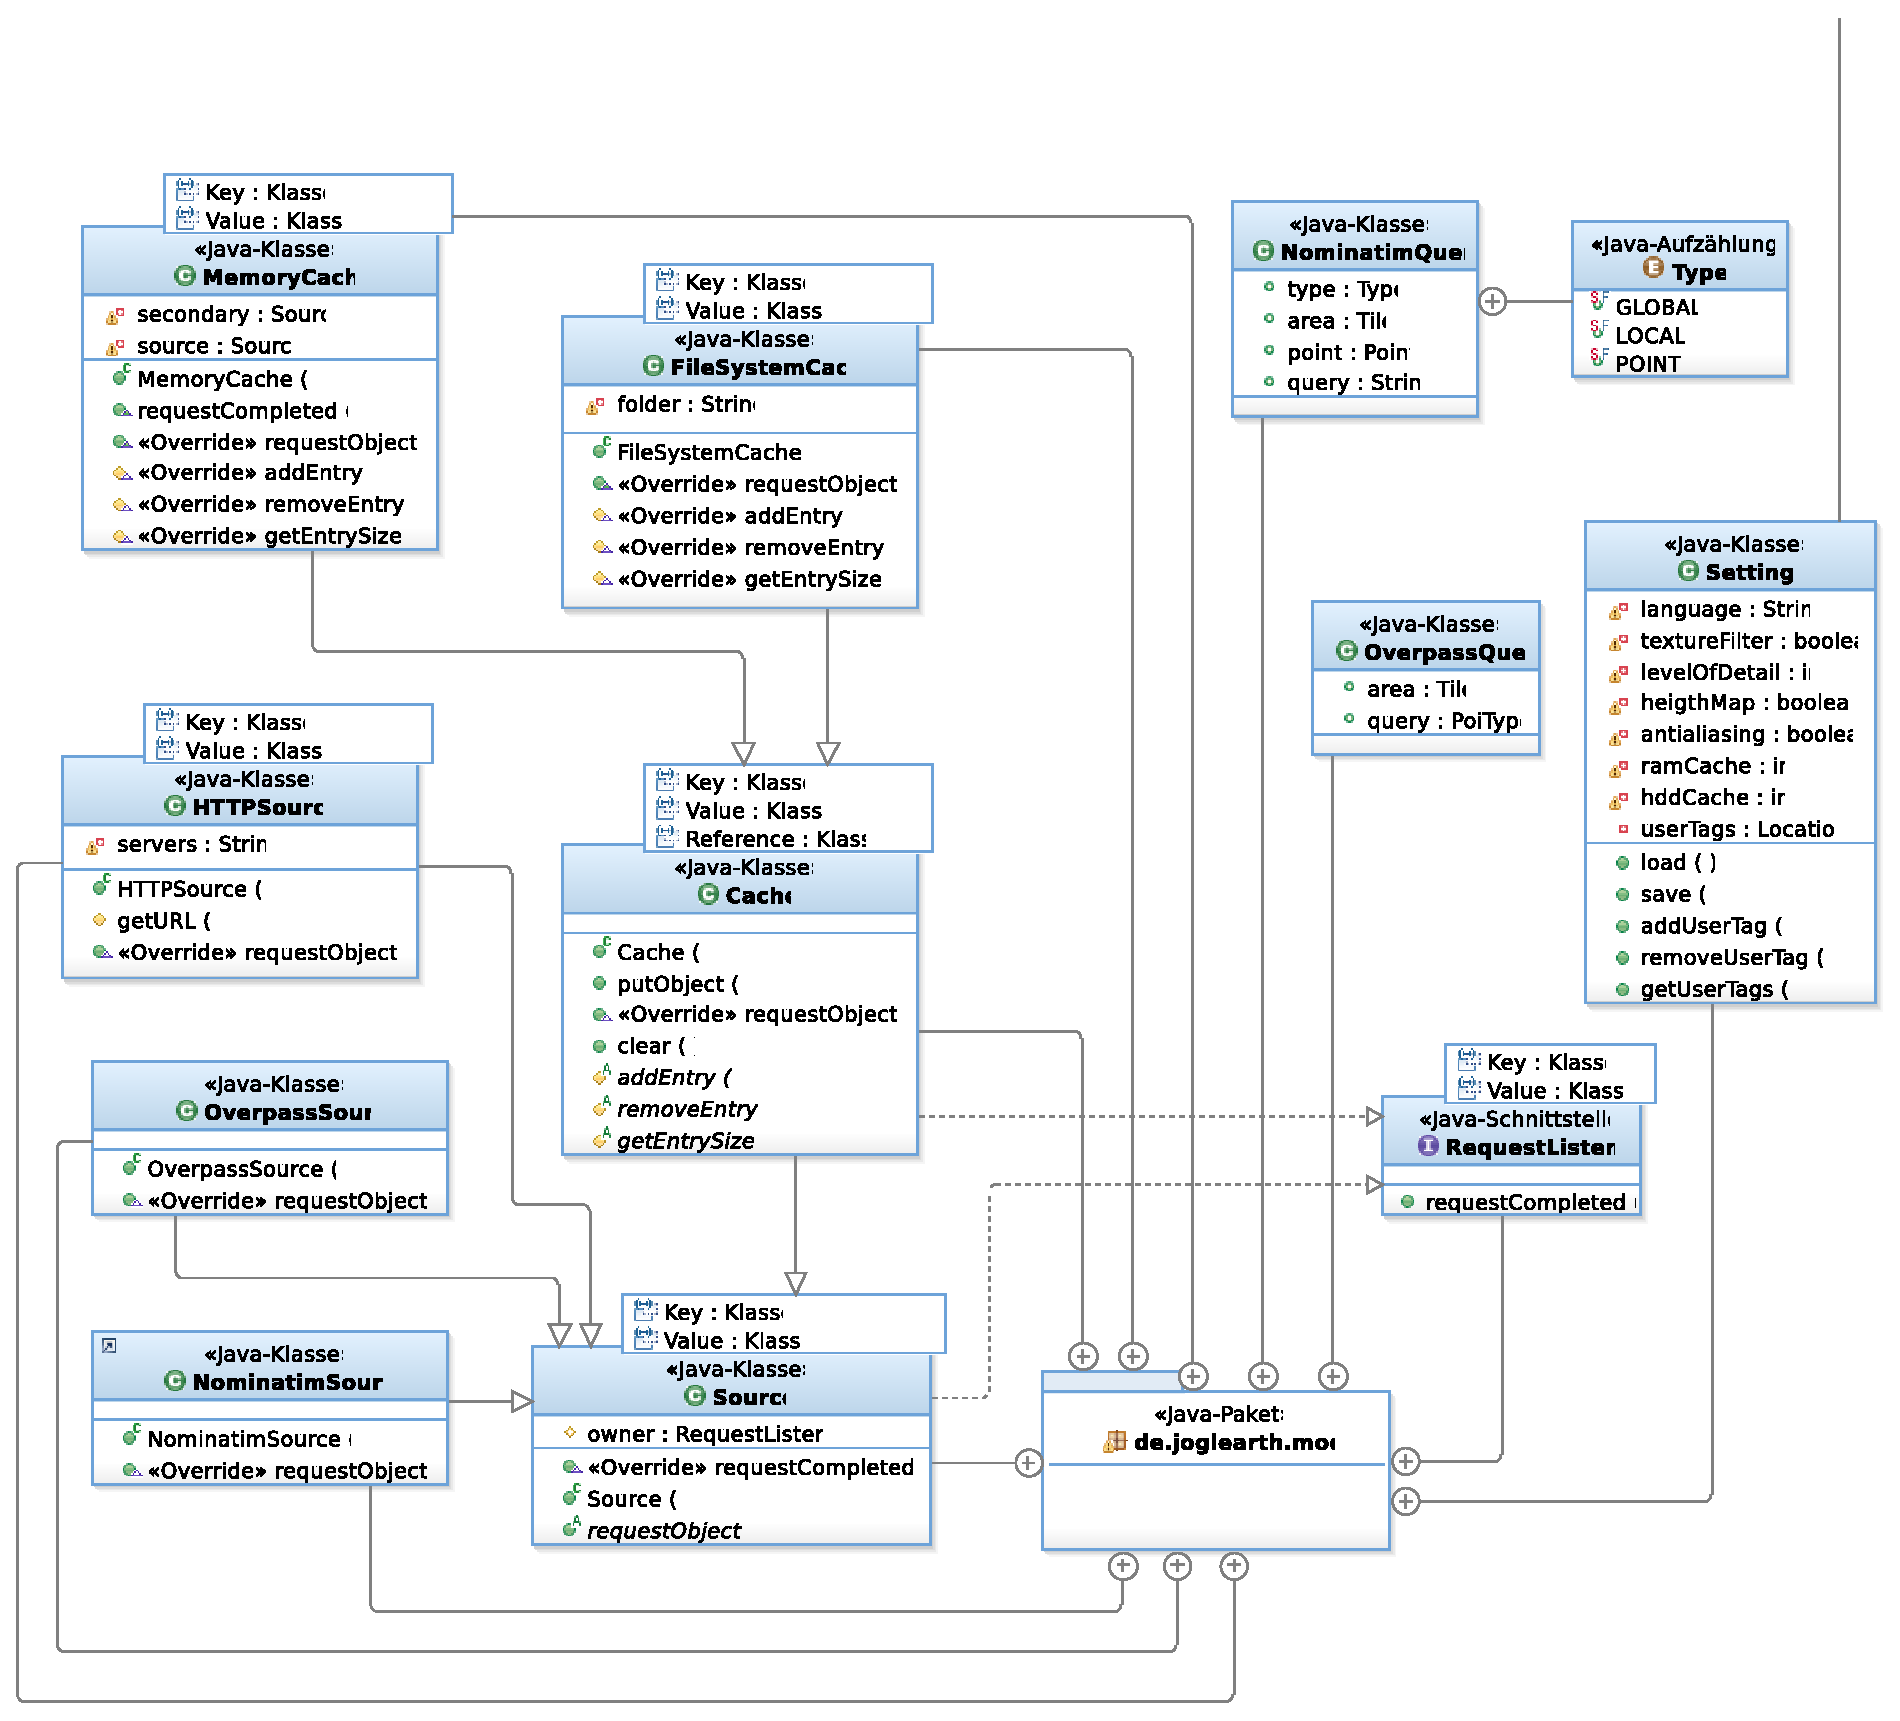
\includegraphics[scale=0.5]{JoglDiagramm_Model.eps}
\vspace{2.0 cm}
\end{figure}

\section{Package View}
\begin{figure}[!htb]
	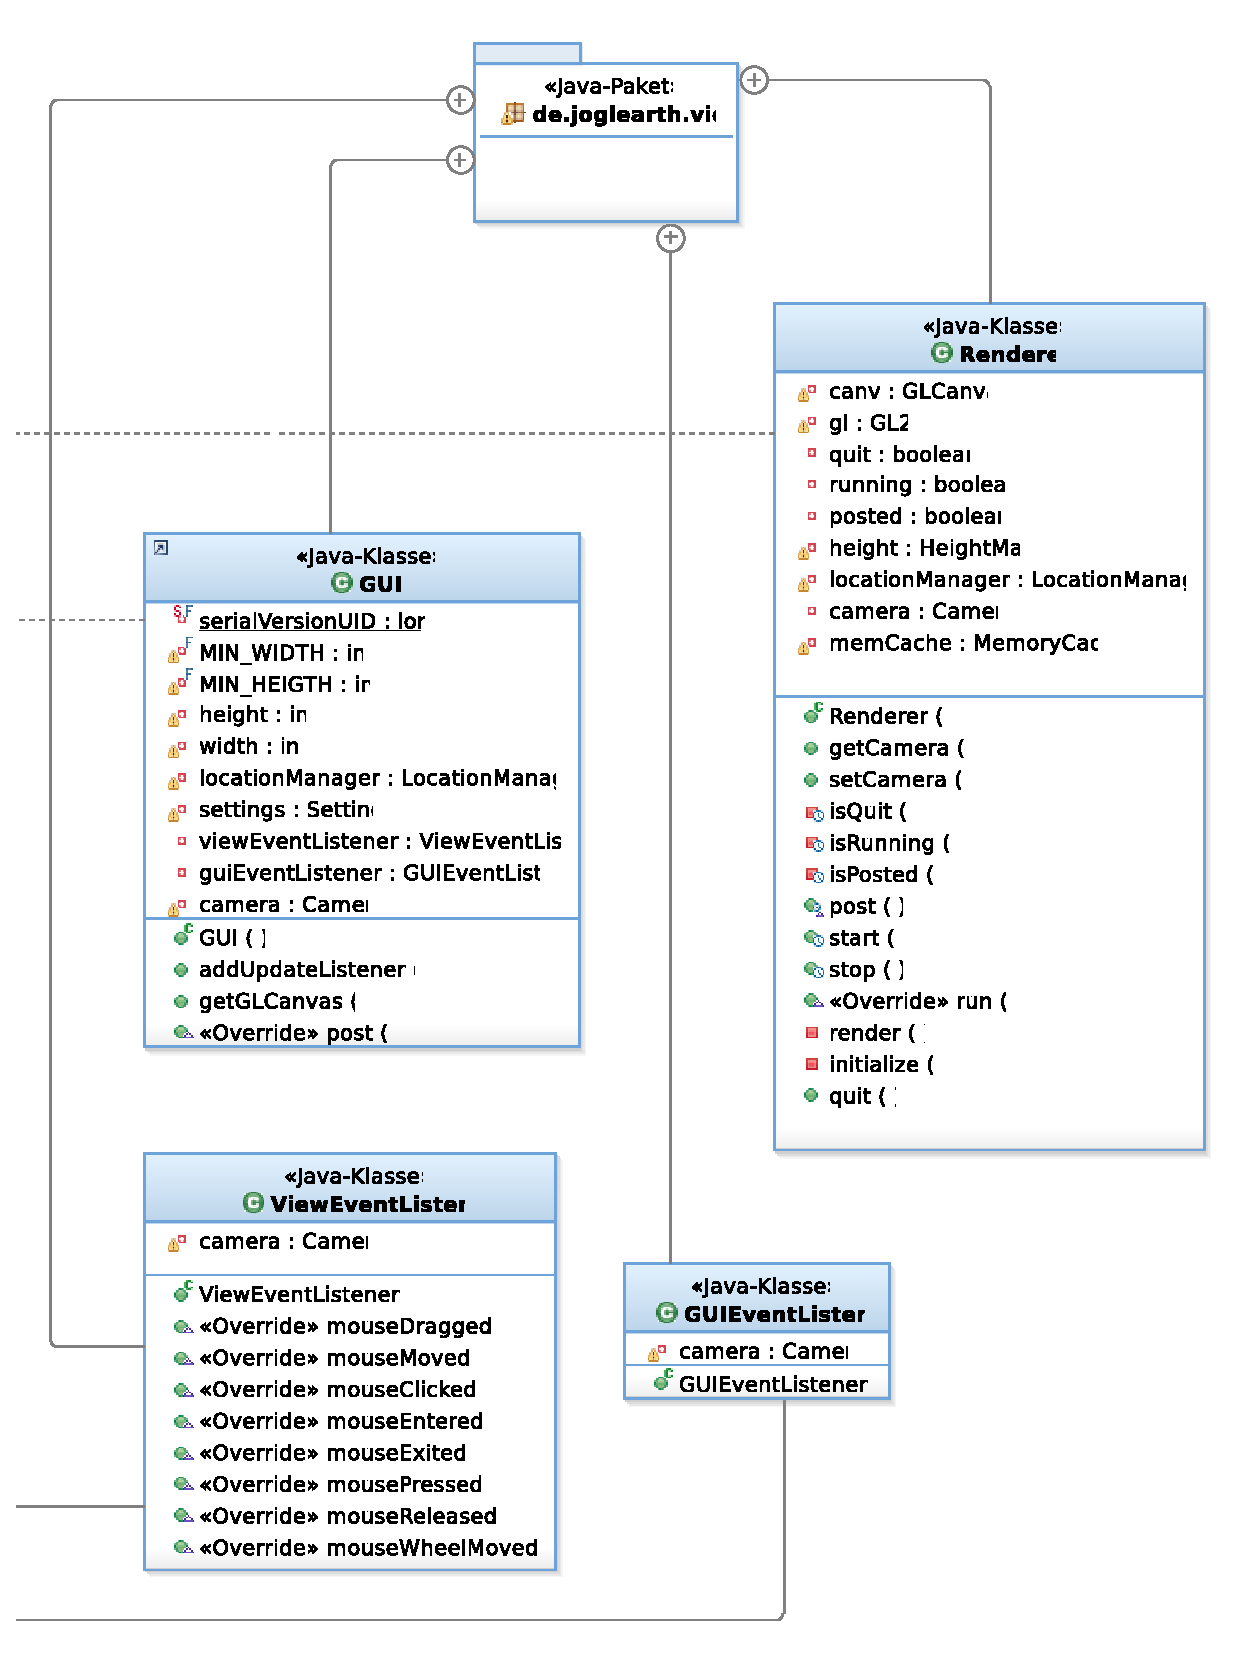
\includegraphics[scale=0.7]{JoglDiagramm_View.eps}
\vspace{2.0 cm}
\end{figure}

\section{Package Controller}
\begin{figure}[!htb]
	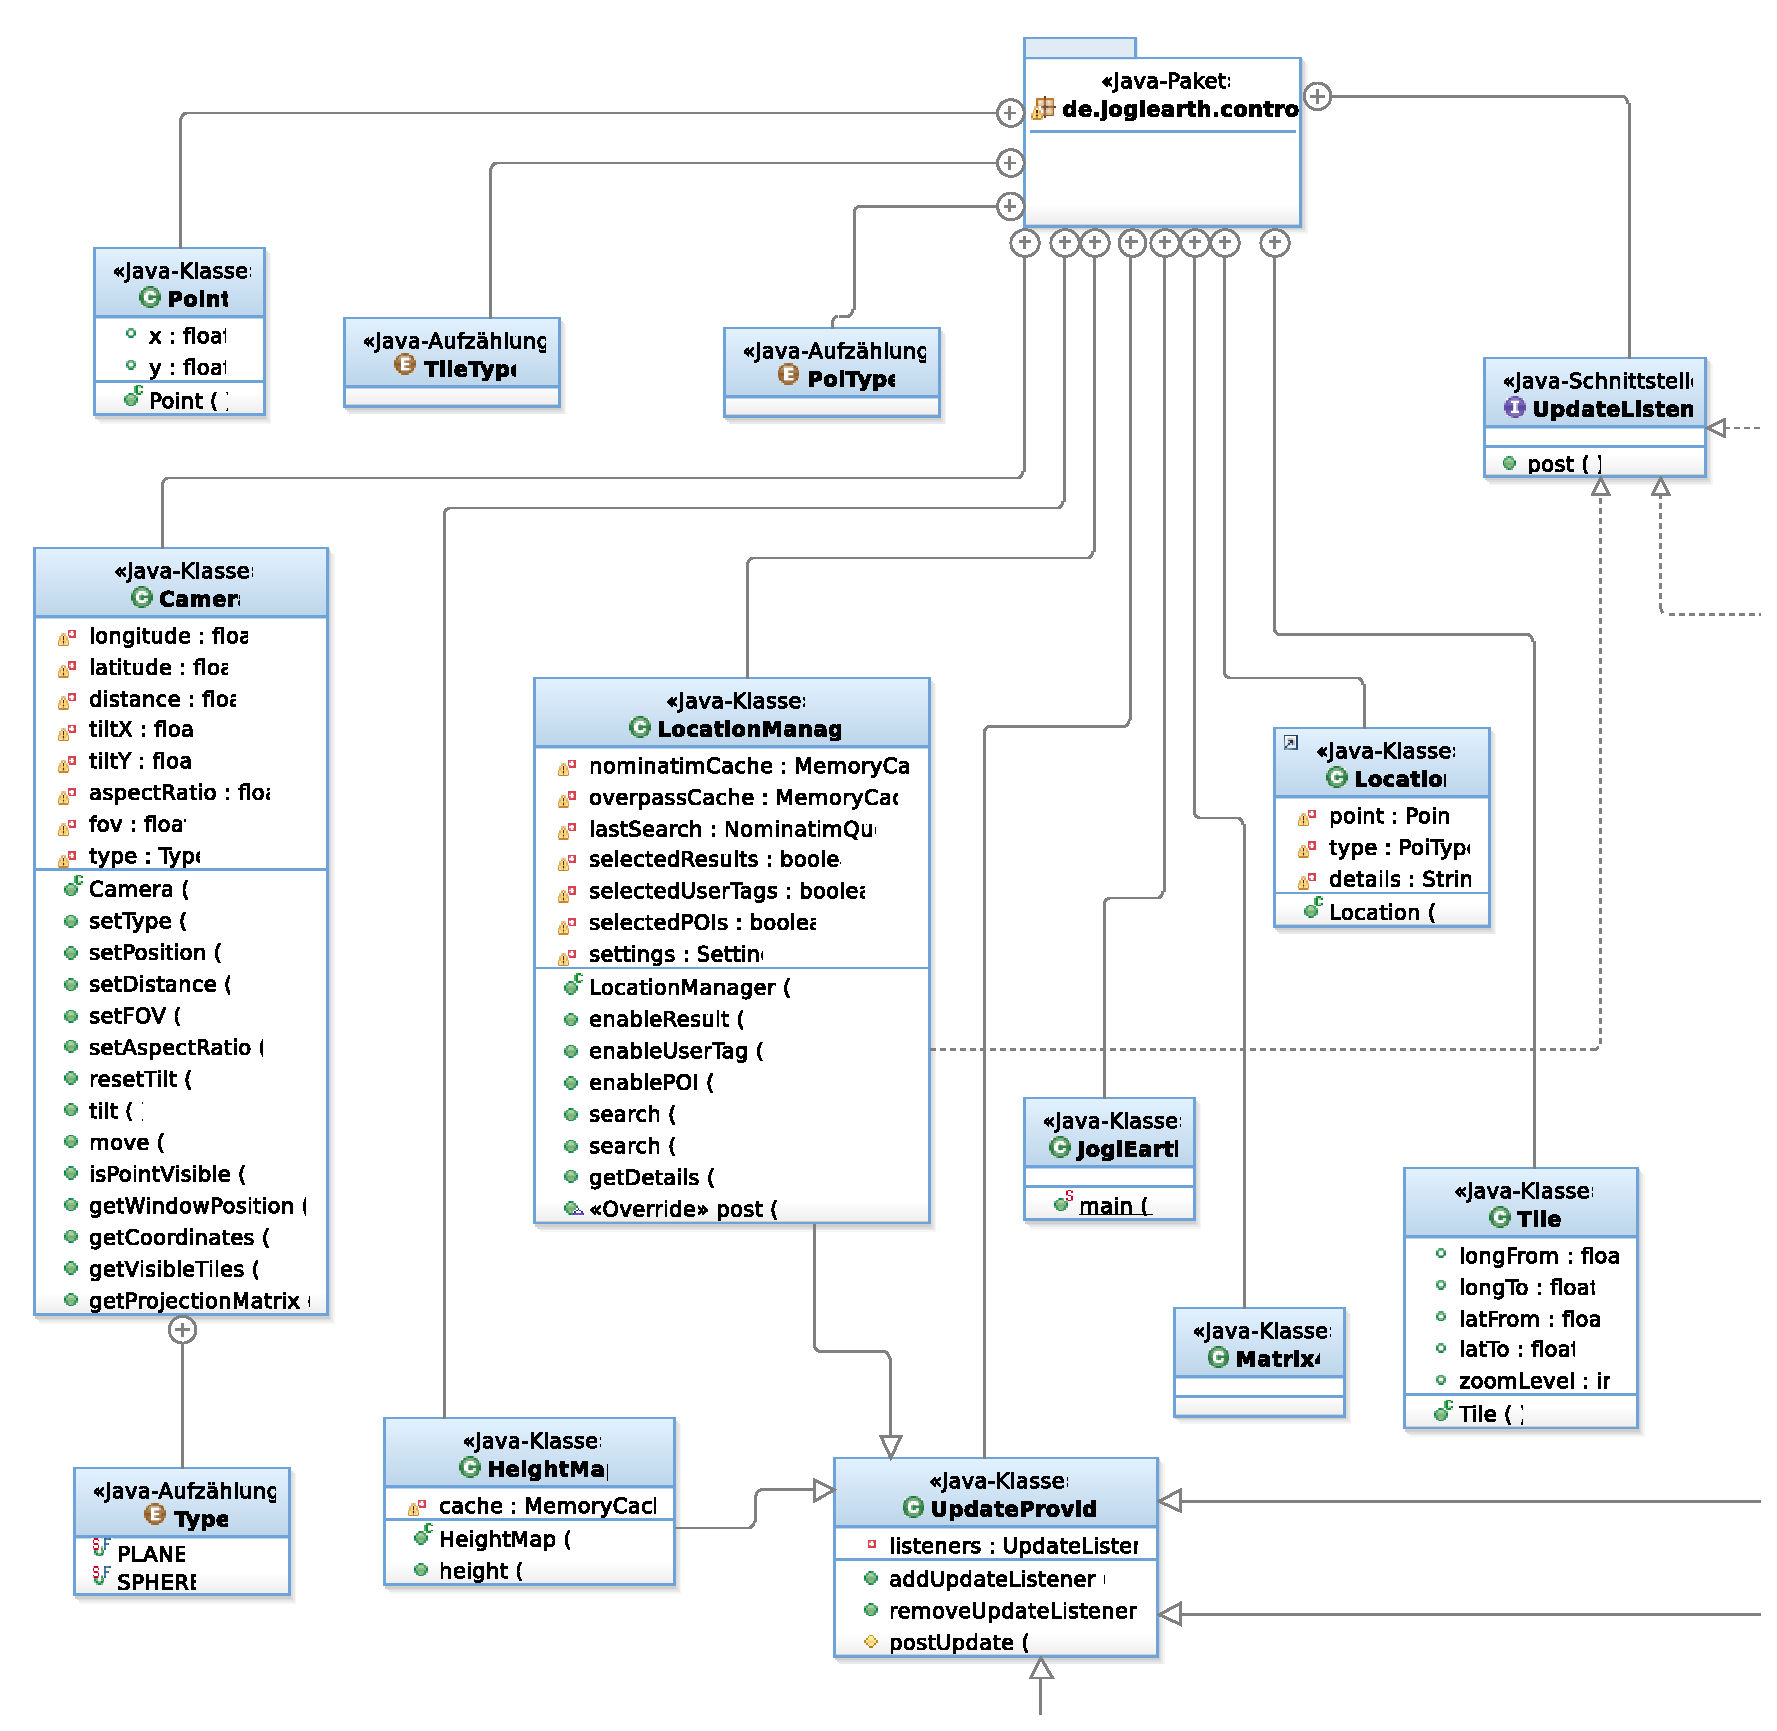
\includegraphics[scale=0.5]{JoglDiagramm_Controller.eps}
\vspace{2.0 cm}
\end{figure}

\chapter{Klassenbeschreibung}

\section{Package Model}

\subsection*{Source}
\begin{lstlisting}
abstract class Source<Key, Value>
implements RequestListener<Key, Value>
\end{lstlisting}
Ist in der Lage, über einen \texttt{Key} identifizierte Objekte asynchron zu beschaffen.
\\


\subsection*{Cache}
\begin{lstlisting}
abstract class Cache<Key, Value, Reference> 
extends Source<Key, Value>
implements RequestListener<Key, Value>
\end{lstlisting}
Bildet die Basis für einen Cache und implementiert eine Verdrängungsstrategie. Die Speicherung der Daten liegt bei der erbenden Klasse.
\\

\subsection*{MemoryCache}
\begin{lstlisting}
class MemoryCache<Key, Value>
extends Cache<Key, Value, Integer>
\end{lstlisting}
Der \textit{MemoryCache} verwaltet einen Zwischenspeicher im RAM. Zudem besitzt er Kenntnis über einen sekundären Cache (beispielsweise einen \textit{FileSystemCache}) und eine Datenquelle, die bei Bedarf angefragt werden können.
\\

\subsection*{FileSystemCache}
\begin{lstlisting}
class FileSystemCache<Key, Value>
extends Cache<Key, Value, String>
\end{lstlisting}
Der \textit{FileSystemCache} speichert Daten im Dateisystem zwischen.
\\

\subsection*{HTTPSource}
Die \textit{HTTPSource} lädt Binärdaten von festgelegten HTTP-Servern.

\subsection*{NominatimSource}
Alle Methoden werden von der Oberklasse \textit{Source} geerbt. Alle Suchanfragen werden von dieser Klasse durchgeführt und die Antworten werden zur Weiterverarbeitung aufbereitet.

\subsection*{OverpassSource}
Alle Methoden werden von der Oberklasse \textit{Source} geerbt. Die anzuzeigenden POIs werden von dieser Klasse angefragt und die Antworten werden zur Weiterverarbeitung aufbereitet.

\subsection*{NominatimQuery}
??

\subsection*{OverpassQuery}
??

\subsection*{Settings}
Die Klasse lädt und speichert alle erforderlichen Einstellungen sowie die vom Benutzer markierten Punkte aus der Datei \texttt{Settings}.
Desweiteren werden die Einstellungen gekapselt und anderen Klassen zugänglich gemacht.


\section{Package View}
\subsection*{GUI}
Die Klasse \textit{GUI} erbt von JFrame und stellt die gesamte grafische Bedienoberfläche dar. Pro Sitzung darf lediglich eine Instanz der \textit{GUI} existieren.

\subsection*{GUIEventListener}
??

\subsection*{ViewEventListener}
??

\subsection*{Renderer}
??


\section{Package Controller}
\subsection*{Camera}


\subsection*{HeightMap}


\subsection*{UpdateProvider}


\subsection*{Location}


\subsection*{LocationManager}


\subsection*{Tile}


\subsection*{Point}


\subsection*{Matrix4}


\subsection*{JoglEarth}
Die Klasse stellt die \textit{Main} Methode bereit.


\chapter{Sequenzdiagramme}




\chapter{Beschreibung der Interfaces}

\section{Package Model}

\subsection*{RequestListener}

\section{Package View}

\section{Package Controller}

\subsection*{UpdateListener}




\chapter{Beschreibung der Enumerations}

\section{Package Model}

\subsection*{NominatimQuery.Type}

\section{Package View}

\section{Package Controller}

\subsection*{TileType}
\subsection*{PoiType}
\subsection*{Camera.Type}

\chapter{Designpatterns}
\section{Adapter Pattern}
Das \textit{Adapter Pattern} ist ein Strukturmuster. \\
Es dient zur Übersetzung einer Schnittstelle in eine andere. \\ Dieses Pattern findet Anwendung bei den \textit{Mouse- und Key"-listenern}, welche in der Benutzeroberfläche implementiert werden. \\ Ziel ist es den Quellcode übersichtlich zu halten. Aus diesem Grund werden nur die benötigten Methoden der Listener überschrieben. Alle nicht erforderlichen Methoden werden ignoriert.

\section{Chain of Responsibility Pattern}
Das \textit{Chain of Responsibility Pattern} (bzw. Zuständigkeitskette) ist ein Verhaltensmuster. \\
Hierbei werden mehrere Objekte hintereinander verkettet um gemeinsam eine eingehende Anfrage bearbeiten zu können. Dafür wird eine Anfrage entlang der Kette durchgereicht, bis ein Objekt die Anfrage beantworten kann. \\ Es findet Anwendung beim Speichermanagement. Eine Anfrage für eine benötigte Ressource wird immer an den \textit{memoryCache} gestellt. Die Anfrage wird entsprechend der Kette (siehe Abbildung) durchgereicht bis sie bearbeitet werden kann. \\ Ziel ist  die Entkopplung des Auslösers einer Anfrage mit seinem Empfänger.

\section{Data Transfer Object}
Das \textit{Data Transfer Object} ist ein Muster für objektrelationale Abbildung. \\
Hierbei werden mehrere Daten gebündelt als ein Objekt übertragen. \\ Es findet Anwendung bei Suchergebnissen und der Anfrage nach POIs. Alle Datensätze werden dann gebündelt übergeben und nicht jede Information seperat. \\ Ziel ist es die Daten zu strukturieren bzw. vollständig gruppierte Information zu einer Anfrage zu erhalten.

\section{Iterator Pattern}
Das \textit{Iterator Pattern} ist ein Verhaltensmuster. \\ Hierbei wird die verwendete Datenstruktur elementweise durchlaufen, ohne deren interne Anordnung preiszugeben.\\ Es findet Anwendung ... \\ Ziel ist es die eingesetzten Datenstrukturen effizient zu durchsuchen.

\newpage
\section{Mediator Pattern}
Das \textit{Mediator Pattern} ist ein Verhaltensmuster. \\ Hierbei fungiert der Vermittler als Kommunikationsschnittstelle zwischen Objekten in einem komplexen System. \\ Es findet mehrfache Anwendung im gesamten Programm, wie beispielsweise beim Speichermanagement, beim Rendering, usw. \\ Ziel ist lockere Kopplung. Es sollen nicht alle Objekt voneinander Kenntnis besitzen.

\section{Model-View-Controller (MVC) Pattern}
Das \textit{Model-View-Controller Pattern} ist ein Architekturmuster. \\
\begin{figure}[ht]
\begin{centering}
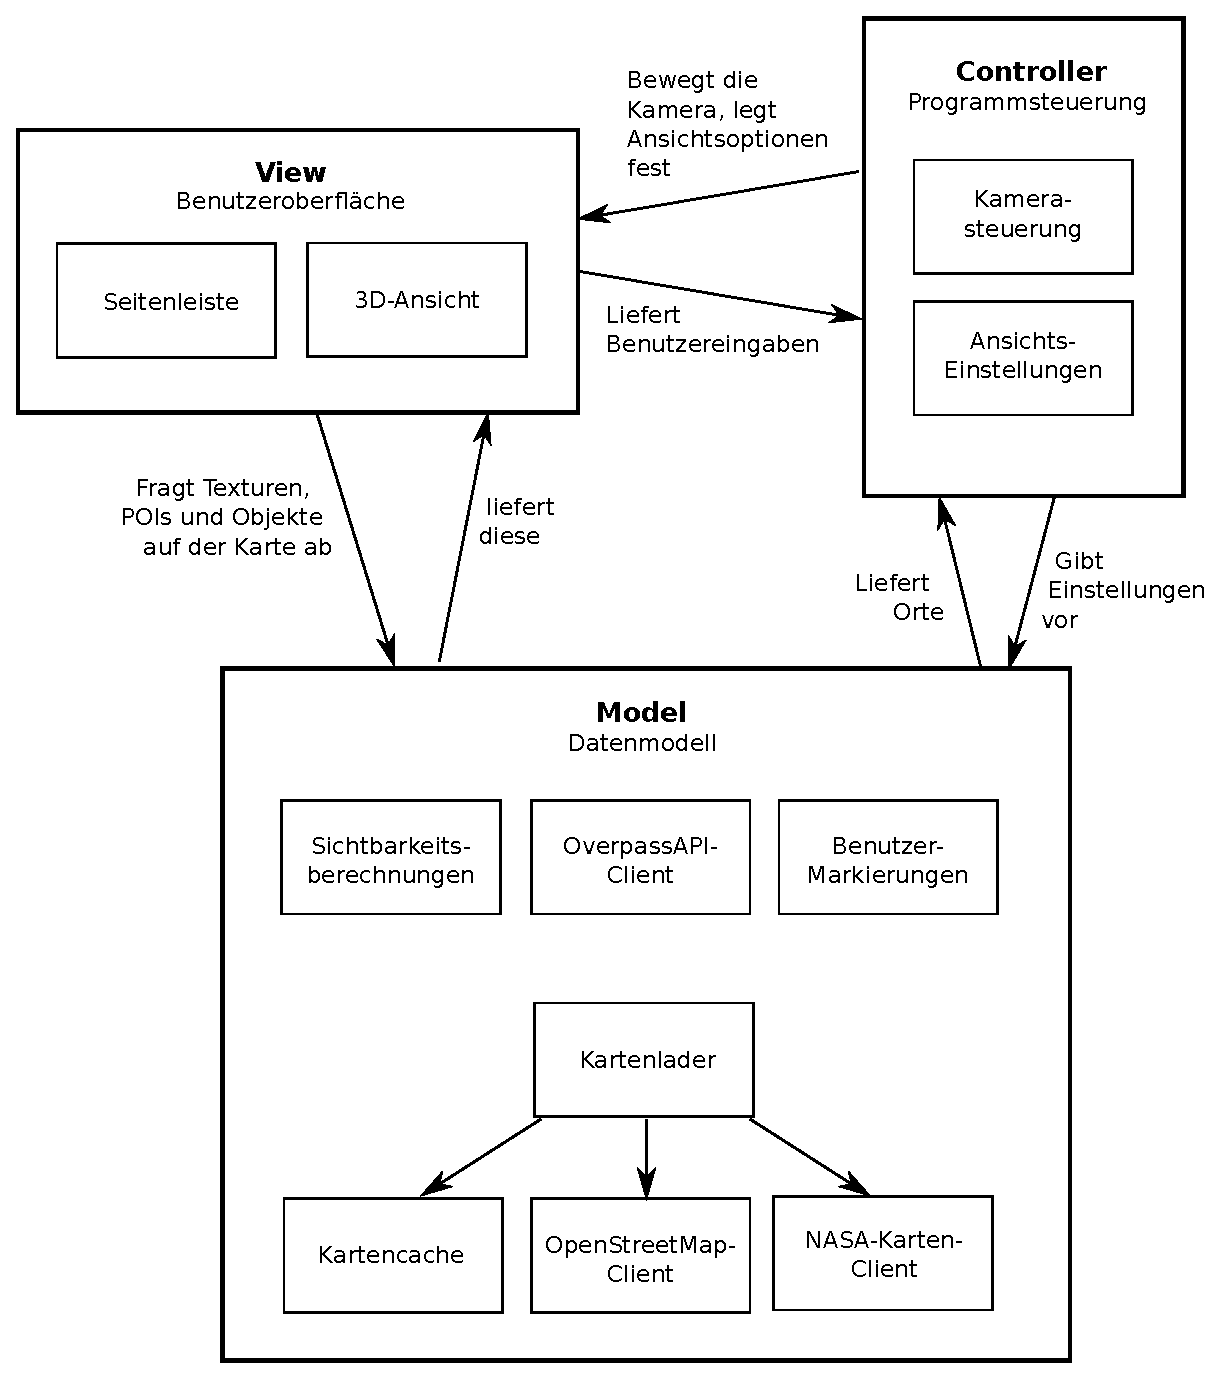
\includegraphics[scale=0.5]{ModelViewController.eps}
\caption{Das Model-View-Controller Pattern}
\end{centering}
\end{figure}



\section{Multiton Pattern}
Das \textit{Multiton Pattern} ist ein Erzeugungsmuster. \\ Hierbei wird sichergestellt, dass mehrere Instanzen eines Objekts existieren dürfen. Eine eindeutige Zuordnung wird geregelt durch Vergabe eines Schlüssels. \\ Es findet Anwendung bei den \textit{RequestListenern} ???? \\ Ziel ist parallele Anfragestellung und -beantwortung.

\section{Observer Pattern}
Das \textit{Observer Pattern} ist ein Verhaltensmuster. \\ Hierbei wird eine Info bei durchgeführten Änderungen am Objekt an alle abhängigen Komponenten weitergegeben. \\ Es findet Anwendung ... jede Menge Observer \\ Ziel ist lose Kopplung und zudem werden die abhängigen Objekte automatisch über Änderungen in Kenntnis gesetzt.

\section{Singleton Pattern}
Das \textit{Singleton Pattern} ist ein Erzeugungsmuster. \\ Hierbei wird sichergestellt, dass genau eine einzige Instanz eines Objekts existiert. \\ Es findet Anwendung bei der Benutzeroberfläche, von der nur eine Instanz existieren darf. \\ Ziel ist eine sichergestellte Zugriffskontrolle auf das Objekt. 




\chapter{Qualitätsmerkmale}
\section{Entwurfsqualität}
Bei der Qualität des Entwurfs beziehen wir uns auf \textit{Robert Cecil Martins} Merkmalsdefinitionen \footnote{Robert Cecil Martin (2002). Agile Software Development: Principles, Patterns and Practices. Pearson Education.} die im Folgenden erläutert werden.

\subsection*{Anzahl an Klassen und Interfaces}
Die Anzahl aller Klassen inklusive abstrakter Klassen (sowie Interfaces) im gesamten Paket. Es dient als aussagekräftiger Indikator für die Erweiterbarkeit eines Pakets.

\subsection*{Afferente Kopplung}
Die Abhängigkeit anderer Pakete von einem Paket ist ein Maß für dessen Verantwortlichkeiten und dessen Einfluss.

\subsection*{Efferente Kopplung}
Die Abhängigkeit eines Pakets von anderen Paketen ist ein Maß für die Unselbstständigkeit dieses Pakets.

\subsection*{Abstraktheit}
Der Anteil abstrakter Klassen (sowie Interfaces) an allen Klassen im Paket ist ein Indikator für die Abstraktheit eines Pakets.

\subsection*{Stabilität}
Das Verhältnis von afferenter Kopplung zur gesamten Kopplung gibt Auskunft über die Resilienz gegenüber Änderungen eines Pakets.

\subsection*{Balance von Abstraktion und Abhängigkeit}
Der Abstraktionsgrad der Klassen sollte in etwa deren Unabhängigkeit von anderen Klassen entsprechen. Bei Erfüllung der Anforderung spricht man von optimaler Balance.

\subsection*{Kohäsion}
Als Ergänzung zu Martin's Definitionen, welche sich nur auf das Zusammenspiel zwischen den Paketen bezieht, wird zudem die Kohäsion berücksichtigt.\\

Kohäsion ist der Versuch, zusammenhängende Programmstrukturen in einer Klasse zusammenzuführen, um z.B. nachträgliche Änderungen auf lokale Anpassungen des Codes zu beschränken.


\section{Gütekriterien nach ISO/IEC 9126}
\subsection*{Funktionalität}
Funktionalität beinhaltet Angemessenheit, Richtigkeit, Interoperabilität, Ordnungsmäßigkeit und Sicherheit.

\subsection*{Zuverlässigkeit}
Eine Menge von Merkmalen, die sich auf die Fähigkeit einer Software/eines Systems beziehen, ihr/sein Leistungsniveau unter festgelegten Bedingungen über einen festgelegten Zeitraum oder über eine festgelegte Anzahl von Transaktionen zu bewahren. [ISO 9126]

\subsection*{Benutzbarkeit}
Die Fähigkeit eines Softwareprodukts, unter spezifizierten Bedingungen für einen Benutzer verständlich, erlernbar, anwendbar und attraktiv zu sein. [ISO 9126]

\subsection*{Effizienz}
(1) Die Fähigkeit eines Softwareprodukts, unter festgelegten Bedingungen eine angemessene Leistung zu erbringen, bezogen auf den Umfang der eingesetzten Betriebsmittel. [ISO 9126]

\subsection*{Änderbarkeit}
Mit Änderbarkeit bezeichnet man den Aufwand, der zur Durchführung bestimmter Änderungen notwendig ist. Änderungen können Korrekturen, Verbesserungen oder Anpassungen an Änderungen der Umgebung, der Anforderungen und der funktionalen Spezifikation einschließen. [ISO 9126]

\subsection*{Portabilität}
Portabilität oder Übertragbarkeit ist die Eignung einer Software, von einer Umgebung in eine andere übertragen zu werden. Diese Umgebung kann die organisatorische Umgebung, Hardware- oder Software-Umgebung einschließen. [ISO 9126]


\end {document}